\begin{frame}{メッシュ切設定の概要}
  %
   \begin{columns}[t]
    \begin{column}{0.6\textwidth}
      <今回のメッシュ切設定の概要>
      \begin{itemize}
        \item[(1)]<1-> 全体のメッシュサイズを4mmに設定
        \item[(2)]<2-> 全体のメッシュを「TransFinite」に設定
	\item[(3)]<3-> 厚み方向のメッシュサイズを1mm(20分割)
		       に設定
        \item[(4)]<4-> メッシュ作成!
        \item[(5)]<5-> 板厚方向のメッシュが全立体に伝搬する
      \end{itemize}
    \end{column}
    \begin{column}{0.4\textwidth}
      \vspace{-7mm}
      \begin{figure}[htbp]
        \begin{center}
          \begin{overlayarea}{7cm}{15cm}
            \only<1>{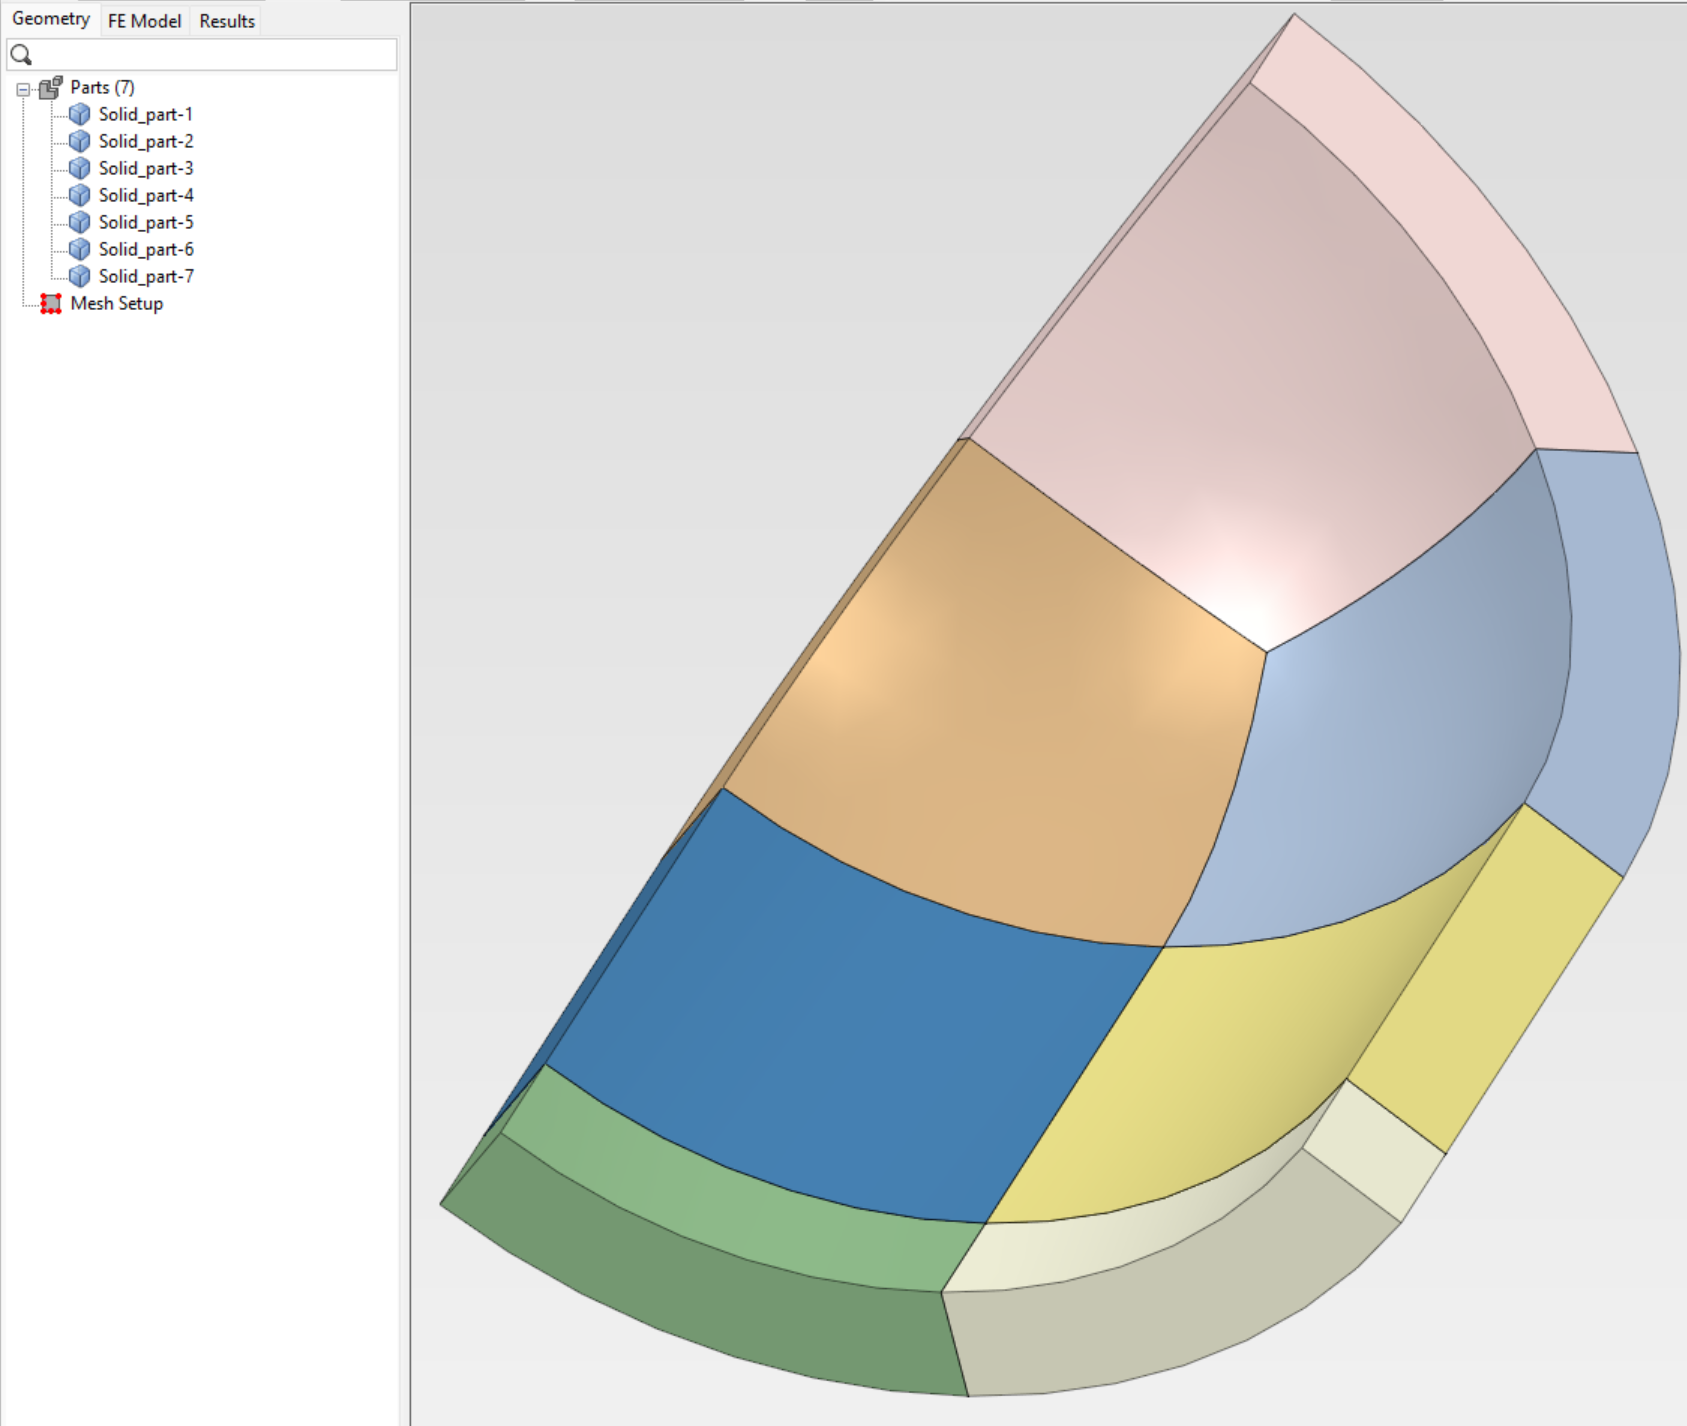
\includegraphics[keepaspectratio,scale=0.30]{images/sc4.png}}
            \only<2>{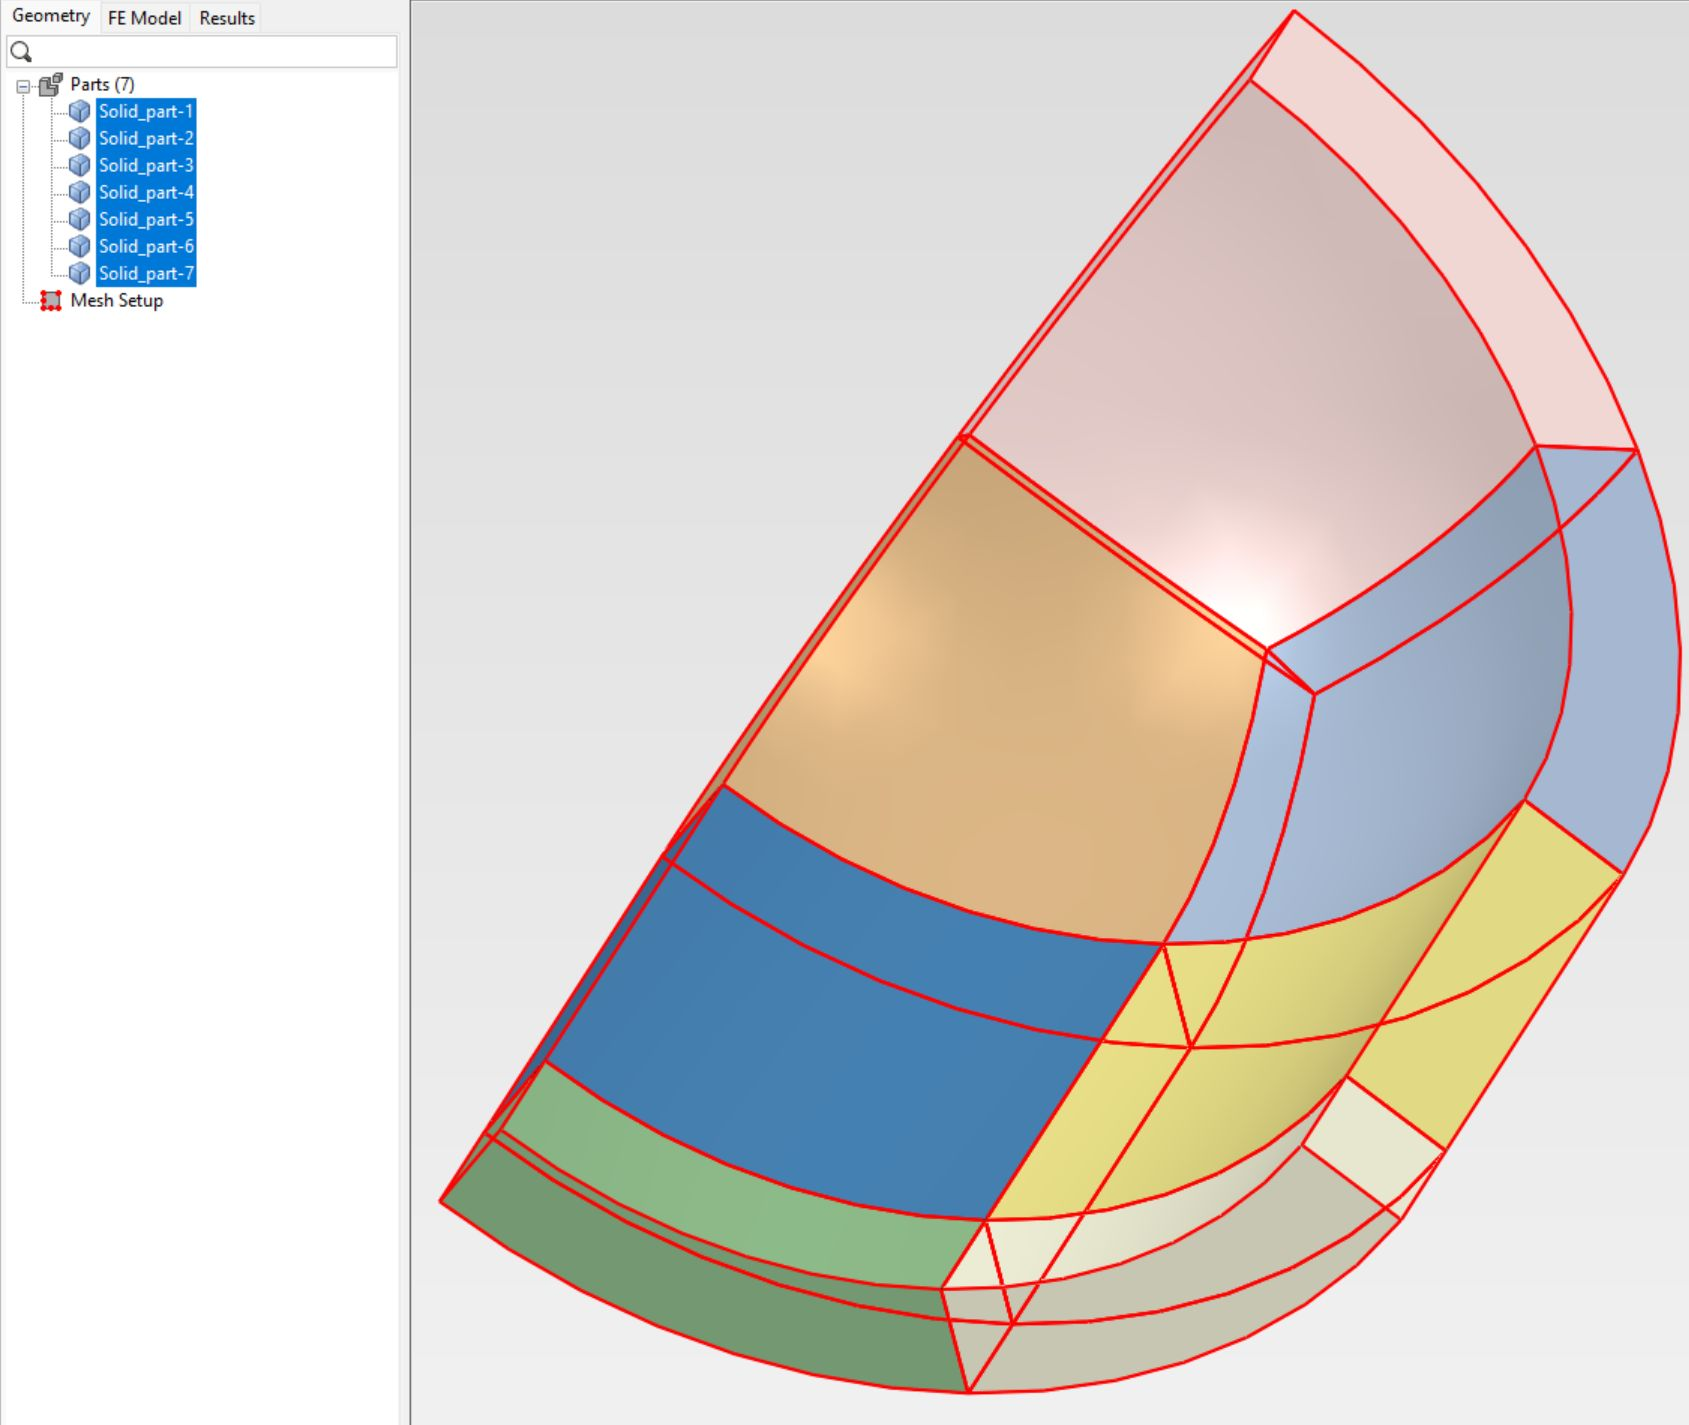
\includegraphics[keepaspectratio,scale=0.30]{images/sc5.png}}
            \only<3->{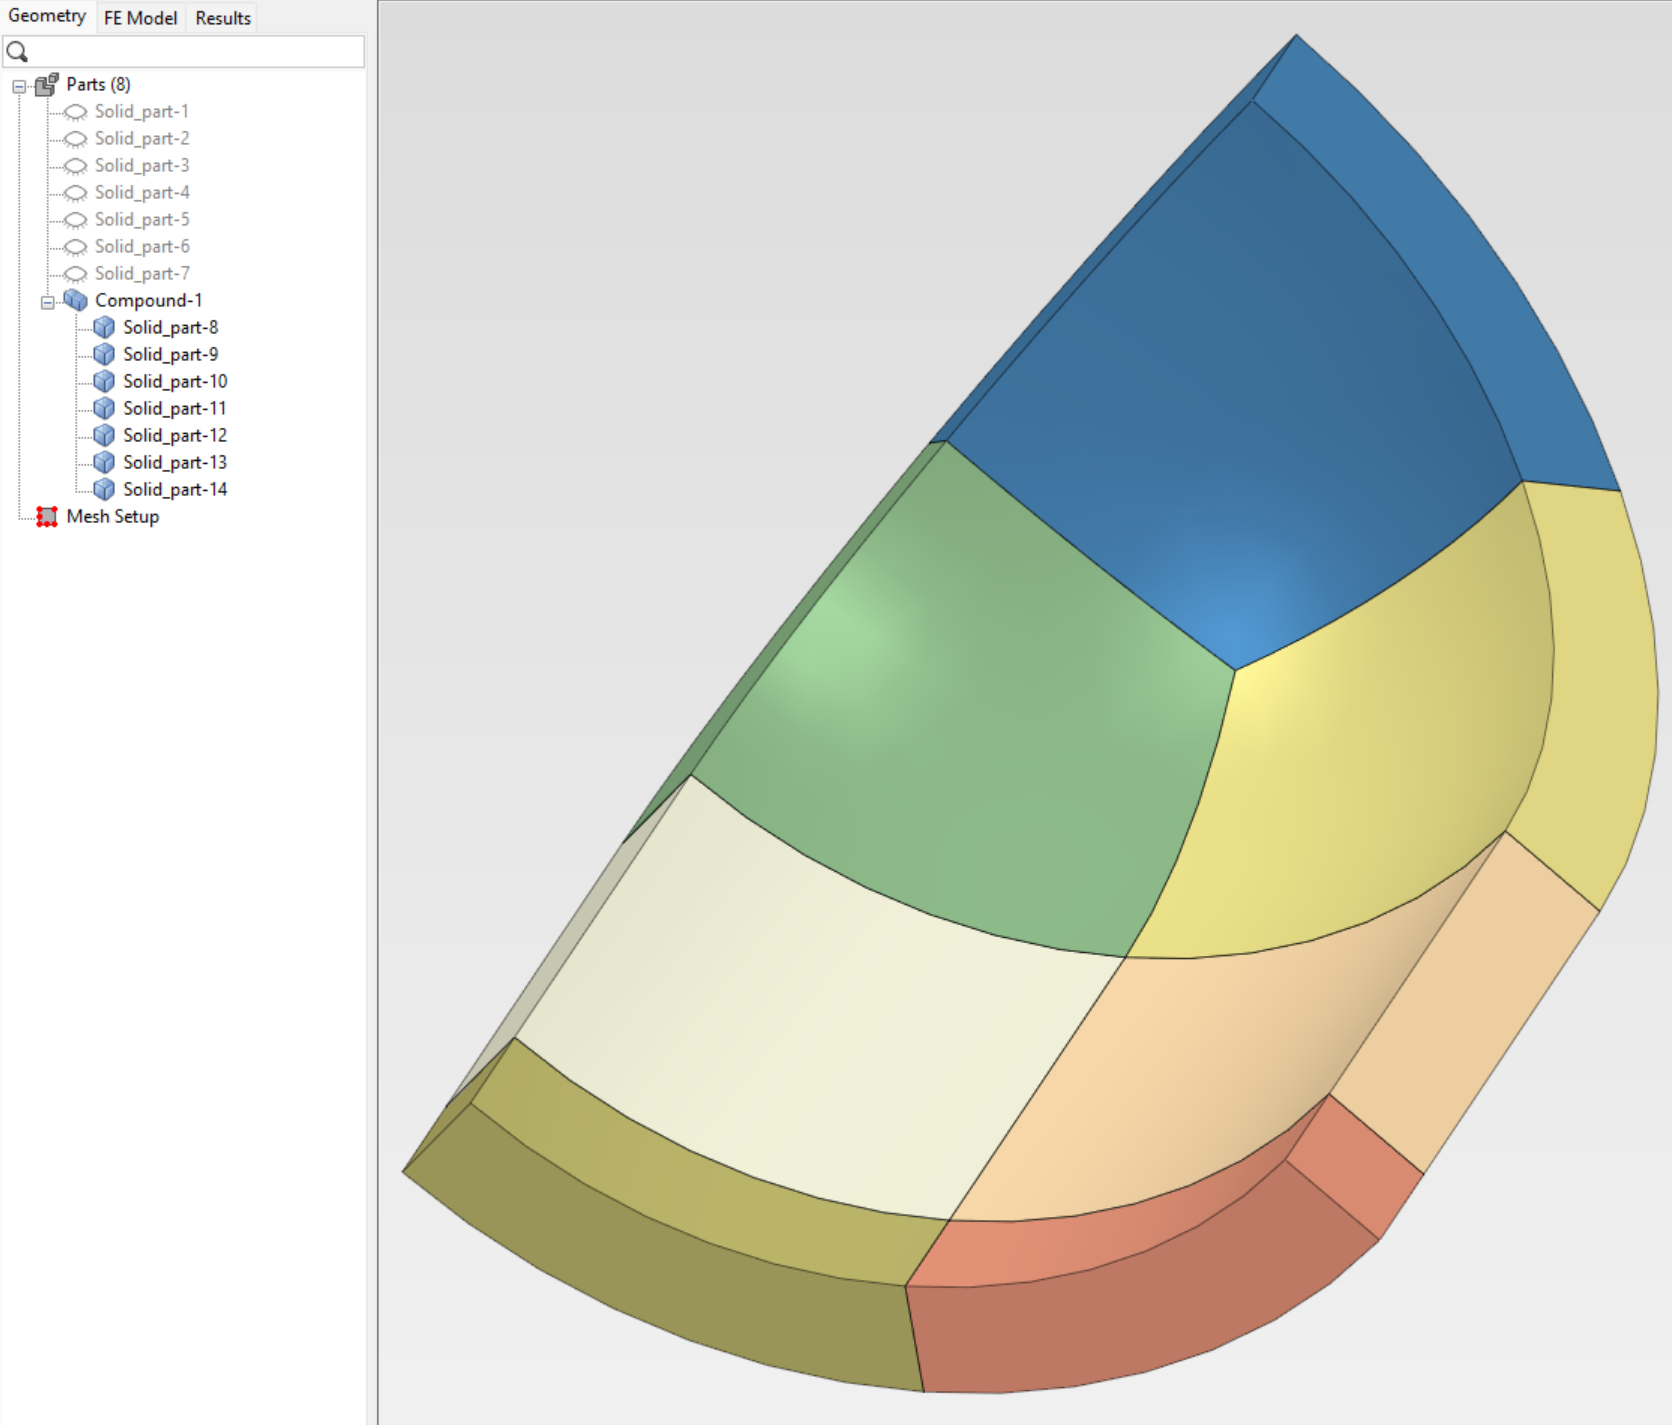
\includegraphics[keepaspectratio,scale=0.30]{images/sc6.png}}
            \caption{メッシュ設定の概要}
          \end{overlayarea}
        \end{center}
      \end{figure}
    \end{column}
  \end{columns}
  \only<1>{
    \begin{textblock*}{140pt}(210pt,60pt)
      \begin{tikzpicture}
         \node[rectangle,fill=cud_yellow,text width=70pt,text centered,rounded corners,minimum height=40pt](s) at (1cm,1cm) { \scriptsize 7つの立体が\\取り込まれる};
         \draw[->, draw=cud_red, line width=1pt] (10pt,50pt) -- (30pt,110pt);
      \end{tikzpicture}
    \end{textblock*}
  }
  \only<3>{
    \begin{textblock*}{100pt}(210pt,90pt)
      \begin{tikzpicture}
         \node[rectangle,fill=cud_yellow,text width=70pt,text centered,rounded corners,minimum height=40pt](s) at (1cm,1cm) { \scriptsize ひとかたまりの\\形状となる};
         \draw[->, draw=cud_red, line width=1pt] (20pt,50pt) -- (40pt,130pt);
      \end{tikzpicture}
    \end{textblock*}
  }
\end{frame}
